%!TEX root =    statphys_main.tex

\chapter{Renormalization Group}

In this chapter we will have a look at the Ising model from a different point of view. After having presented some ways to analytically approach the solution of the Ising model in both 1d and 2d cases, it will now be our aim to make statements about how the spins in such a system correlate to each other, specifically over longer distances than just nearest-neighbour correlation. To obtain these solutions we will make use of a certain iterative renormalization scheme for the partition function.

The general idea for this scheme will be to trace out the effect of designated sites in our Ising-chain, namely, in the 1d case, by marginalizing the probability density function over all odd-labeled sites in the chain. Repeating this process (and thus, further tracing out the effect of some spin sites) will allow us to gain insight into the behaviour of the Ising model in long-range cases.

\section{1D Ising}

We discuss and motivate the basic ideas of the renormalization group (RNG) approach in terms of the 1d Ising model  
%
\begin{align}\label{eq:}
  H = -J \sum_{ i =1}^{N} s_{i}s_{i+1}
  - h' \sum_{i} s_{i} \;,
\end{align}
%
as every step can be performed analytically.
We assume $N=2^{L}$, which allows us to 
thin out every other spin repeatedly. In addition we assume periodic boundary conditions (pbc), i.e. $s_{N+1}=s_{1}$.
For the partition function we need
\begin{align}\label{eq:rng_ising_1d_hamiltonian}
\tilde H := - \beta H &:= 
K\sum_{i} s_{i}s_{i+1} + 
h\sum_{i} s_{i} + N \cdot C\;,
\end{align}
where we have added a constant energy  per site $C$ , as it will become relevant in the renormalization scheme.
The pdf for a spin configuration $\{s\}$ is then given by
\begin{align}\label{eq:RNG:Z}
\rho_{N}(s) &= 
\prod_{i=1}^{N}
e^{K s_{i}s_{i+1} + \frac{h}{2} (s_{i}+s_{i+1}) + C}\;.
\end{align}
In the B-field term we have expanded the sum over two different spins $s_i$ and $s_{i+1}$. To avoid the double counting of these spins, the factor $\frac{1}{2}$ is introduced. As we will see, writing the sum like this turns out to be useful later.
Next we want to determine the reduced pdf for "even sites only", which is obtained by   tracing out the  spins on the odd sites. To this end we rewrite $\rho_{N}$ as follows (starting again from the form of \autoref{eq:rng_ising_1d_hamiltonian})
\begin{align}
\rho_{N}(s) &=\prod_{i=1}^{N} e^{K s_{i}s_{i+1} + hs_{i} + C}\\
&=\prod_{i=1}^\text{even} e^{hs_{i} + 2C}
\prod_{i=1}^\text{odd} e^{K \qty(s_{i-1}s_{i} + s_{i}s_{i+1}) + hs_{i} }
\\
&=\prod_{i=1}^\text{even} e^{hs_{i} + 2C}
\prod_{i=1}^\text{odd} e^{\qty(K \qty(s_{i-1} + s_{i+1}) + h) s_{i} }
\end{align}
%
The product sum over the $hs_i$ is simply split up into the odd and even components. The product sum over $s_is_{i+1}$ is carried out only for odd values of $i$ - in order not to loose any factors, both directions $s_{i+1}$ and $s_{i-1}$ are considered in this term.
Then we obtain by the marginalization of $\rho_N$
\begin{align}\label{eq:RNG:Z2}
\rho_\text{even} &= 
\bigg( \prod_{i}^\text{odd}\sum_{s_{i}=\pm 1}
\bigg)
\rho_N(s)\\
&=\bigg( \prod_{j}^\text{even} e^{h s_{j} + 2 C}   \bigg)
\bigg( \prod_{i}^\text{odd}\sum_{s_{i}=\pm 1}
\bigg)
e^{\qty(K (s_{i-1}+ s_{i+1}) + h )s_{i}}
\;.
\end{align}
%
This marginal pdf is required, if we want to calculate the spin-spin correlation for spins on
even sites only. In particular, it allows to compute the spin-spin correlation 
%
\begin{align}\label{eq:}
\langle s_{2i} s_{2(i+1)}\rangle\;.
\end{align}
%
If we repeat the marginalization once more, we obtain a marginal pdf that allows to compute
%
\begin{align}\label{eq:}
\langle s_{4i} s_{4(i+1)}\rangle\;.
\end{align}
%
Hence, the repeated marginalization of half of the sites allows to determine how spin spin-correlations behave on different length scales.
Now we want to really compute \eq{eq:RNG:Z2}.
%
\begin{align}\label{eq:}
\rho_\text{even} &= \bigg( \prod_{i}^\text{even} e^{h s_{i} + 2 C}   \bigg)
\bigg( \prod_{i}^\text{odd}
\sum_{s_{i}=\pm 1}
e^{s_{i}\big(K (s_{i-1}+ s_{i+1}) + h\big)}\bigg)\\
&=\bigg( \prod_{i}^\text{even} e^{h s_{i} + 2 C}   \bigg)
\bigg( \prod_{i}^\text{odd}
2\;\cosh\big( K (s_{i-1}+ s_{i+1}) + h \big)
\bigg)\\
&= \; \prod_{i}^\text{even} e^{h s_{i} + 2 C + \ln(2)  }
\cosh\big( K (s_{i}+ s_{i+2}) + h \big)\\
&=  \prod_{i}^{N/2} e^{\frac{h}{2} (s_{2i}+s_{2(i+1)}) + 2 C + \ln(2)  }
\cosh\big( K (s_{2i}+ s_{2(i+1)}) + h \big)\;.
\end{align}
%
Next we define $s^{(b)}_{i}=s_{b i}$ and find in particular for $b=2$
%
\begin{align}\label{eq:}
\rho_\text{even}
&= \;\bigg( \prod_{i}^{N/2} e^{\frac{h}{2} (s^{(2)}_{i}+s^{(2)}_{i+1}) + 2 C + \ln(2)  }
\cosh\big( K (s^{(2)}_{i}+ s^{(2)}_{i+1}) + h \big)
\bigg)\;.
\end{align}
%
Finally, we want to express the marginal density formally identically to equation \eqref{eq:RNG:Z}
%
\begin{align}\label{eq:RNG:Z3}
\rho_\text{even}:=\rho_{N/2} &= 
\prod_{i=1}^{N/2}
e^{K' s^{(2)}_{i}s^{(2)}_{i+1} + \frac{h'}{2} (s^{(2)}_{i}+s^{(2)}_{i+1}) + C'}\;,
\end{align}
which is possible, since each factor
%
\begin{align*}
e^{K' s^{(2)}_{i}s^{(2)}_{i+1} + \frac{h'}{2} (s^{(2)}_{i}+s^{(2)}_{i+1}) + C'}
&=
e^{\frac{h}{2} (s^{(2)}_{i}+s^{(2)}_{i+1})+2 C + \ln(2)  }
\cosh\big( K (s^{(2)}_{i}+ s^{(2)}_{i+1}) + h \big)
\end{align*}
%
only depends on $s^{(2)}_{i}+s^{(2)}_{i+1}$, and $s^{(2)}_{i}s^{(2)}_{i+1}$,  for which 
3 different values are possible each, which defines the 3 parameters $K',h',C'$. The corresponding 
conditions are
%
\begin{subequations}
\begin{align}
&s^{(2)}_{i}=s^{(2)}_{i+1}=1:&e^{K'  + h'  + C'} &= e^{h+ 2C + \ln(2)} \cosh(h+2K)
\label{eq:RNG:conda}\\
&s^{(2)}_{i}=s^{(2)}_{i+1}=-1:&e^{K'  - h'  + C'} &= e^{-h+ 2C + \ln(2)} \cosh(h-2K)\label{eq:RNG:condb}\\
&s^{(2)}_{i}=-s^{(2)}_{i+1}:&e^{-K'    + C'} &= e^{2C + \ln(2)} \cosh(h)\label{eq:RNG:condc}
\end{align}	
\end{subequations}
%
From \eq{eq:RNG:condc} we obgtain
%
\begin{align}\label{eq:RNG:cond:app}
e^{C'} &= e^{K' + 2C + \ln(2)} \cosh(h)
\end{align}
%
Insertion in the first two equations yields
\begin{subequations}
\begin{align}
e^{2K'  + h'}\cosh(h) &= e^{h} \cosh(h+2K)
\label{eq:RNG:condap}\\
e^{2K'  - h'}\cosh(h) &= e^{-h} \cosh(h-2K)\label{eq:RNG:condbp}\;.
\end{align}	
\end{subequations}
Multiplication of these  equations yields
\begin{align}
e^{4K' } &= \frac{\cosh(h+2K)\cosh(h-2K)}{\cosh^{2}(h)}
\label{eq:RNG:cond:bpp}\;,
\end{align}	
and division  of these  equations yields
\begin{align}
e^{2h'} &= e^{2h}\frac{\cosh(h+2K)}{\cosh(h-2K)}
\label{eq:RNG:cond:cpp}\;.
\end{align}	
\eq{eq:RNG:cond:app} can alternatively be written as
\begin{align}\label{eq:RNG:cond:app2}
e^{4C'} &= e^{4K'} e^{8C + 4\ln(2)} \cosh^{4}(h)
\end{align}
Along with \eq{eq:RNG:cond:bpp} we obtain
\begin{align}\label{eq:RNG:cond:appp}
e^{4C'} &= \cosh(h+2K)\cosh(h-2K) e^{8C + 4\ln(2)} \cosh^{2}(h)\;.
\end{align}
The equations \ref{eq:RNG:cond:bpp},  \ref{eq:RNG:cond:cpp}, and  \ref{eq:RNG:cond:appp} 
uniquely define the values of $h',K',C'$, which we now denote as 
$h^{(2)},K^{(2)},C^{(2)}$. 
The key finding is that the reduced density matrix  is formally identical to the original one with modified parameters and due to the translational invariance it is actually the same for the even and odd sites. Therefore we denote it simply by $\rho^{(2)}$. Now we can repeat this procedure and obtain $\rho^{(3)}$, which is the reduced density if only every fourth site is retained. The corresponding parameters $h^{(3)},K^{(3)},C^{(3)}$
are related to the parameters $h^{(2)},K^{(2)},C^{(2)}$ of the previous iteration via \eq{eq:RNG:cond:bpp}, \eq{eq:RNG:cond:cpp}, and \eq{eq:RNG:cond:appp}. In general we obtain the iteration scheme
\begin{subequations}\label{eq:iteration}
\begin{align}
e^{4K^{(n+1)} } &= \frac{\cosh(h^{(n)}+2K^{(n)})\cosh(h^{n)}-2K^{(n)})}{\cosh^{2}(h^{n)})}\\
e^{2h^{(n+1)}} &= e^{2h^{(n)}}\frac{\cosh(h^{(n)}+2K^{(n)})}{\cosh(h^{(n)}-2K^{(n)})}\\
 e^{4C^{(n+1)}} &= \cosh(h^{(n)}+2K^{(n)})\cosh(h^{(n)}-2K^{(n)}) e^{8C^{(n)} + 4\ln(2)} \cosh^{2}(h^{(n)})\;
\end{align}
\end{subequations}
The iteration starts with $K^{(1)}=K, h^{(1)}=h$, and $C^{(1)}=C$.
For a first discussion, we consider the case $h=0$, i.e. no external magnetic field. Then the first iteration yields for $h$
\begin{subequations}\label{eq:iteration:h:0}
\begin{align}
e^{2h^{(2)}} &= \frac{\cosh(2K^{(1)})}{\cosh(2K^{(1)})}=1\;,
\end{align}
\end{subequations}
i.e. $h^{(2)}=0$. Hence, $h^{(n)}=0$ for all iteration steps. For the  parameter $K$ we then obtain
the recursion relation
\begin{align}\label{eq:rec:rel:K}
e^{4K^{(n+1)} } &= \cosh^{2}(2K^{(n)}) =
\frac{1}{4}\bigg( e^{2 K^{(n)}}+e^{-2 K^{(n)}} \bigg)^{2}\\
e^{-4K^{(n+1)} } &= 
\frac{4}{\big( e^{2 K^{(n)}}+e^{-2 K^{(n)}} \big)^{2}}
=\frac{4 e^{-4 K^{(n)}}}{\big( 1+e^{-4 K^{(n)}} \big)^{2}}
\end{align}
We introduce the definition  $x^{(n)} = e^{-4 K^{(n)}}$ for which we obtain
%
\begin{align*}
x^{(n+1)} &= f(x^{(n)})\\
f(x) &:=\frac{4 x}{\big( 1+x \big)^{2}}
\end{align*}
%
\begin{figure}[htbp]
\begin{center}
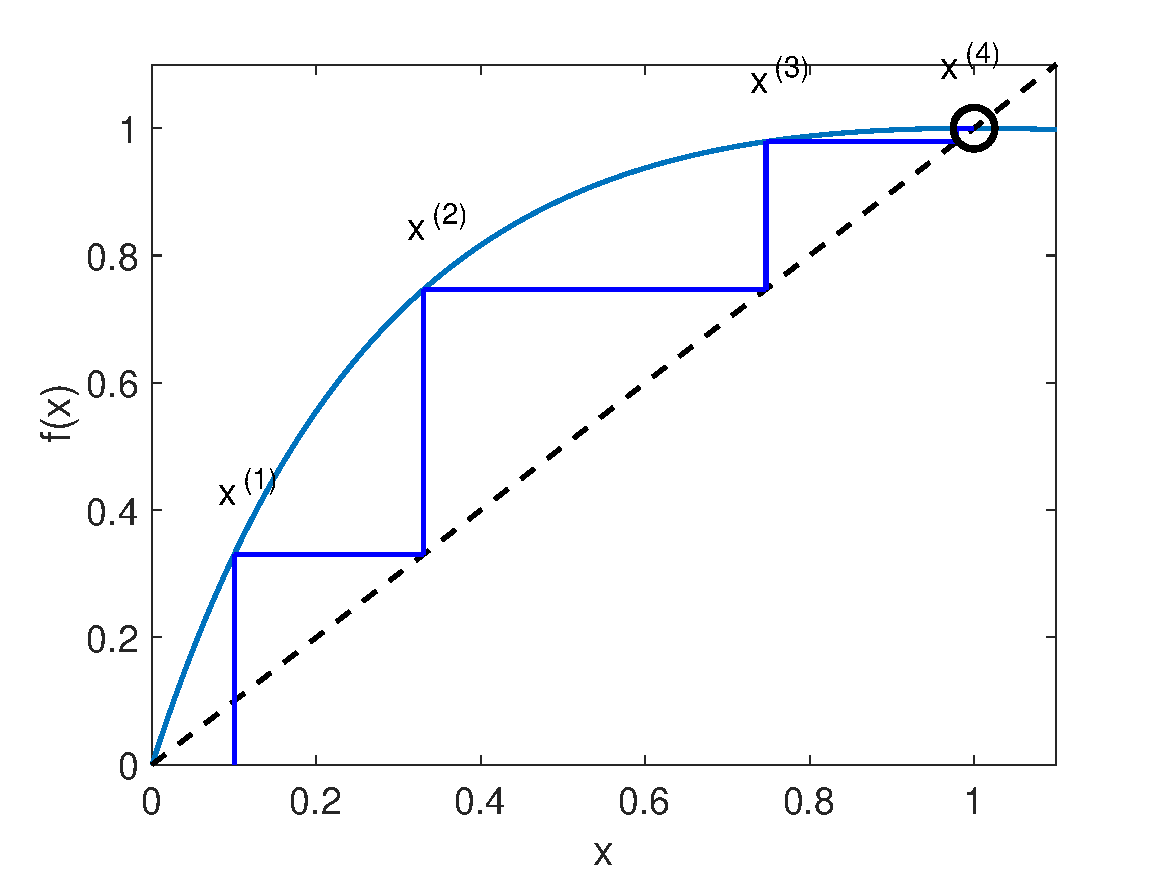
\includegraphics[width=7cm]{NRG_ising}
\caption{{\bf Recursion relation for $x$ in the 1d Ising model. Starting with an arbitrary $x^{(1)}\in(0,1]$ the fixed point is $x^{(\infty)}=1$. Only for
$x^{(1)}=0$ the other fixed point $x^{(\infty)}=0$ is relevant.}}
\label{fig:RNG_ising_x}
\end{center}
\end{figure}
The figure illustrates that if we start the recursion with any value $0< x^{(1)}\le 1$, i.e. $0\le  K< \infty$, which 
corresponds to the parameter of the original physical system, the iteration ends at the fixed point 
$x^{(\infty)}=1$. This means that the physical features (e.g. spin-spin correlation)
for very long distances is equivalent to that of an Ising model with $x=1$, which corresponds to $K=0$. This fixed point is called {\em high temperature fixed point}, as
$x=1$, or rather $K=0$ is also obtained for $T\to \infty$ ($\beta\to 0$).
The 1d Ising model considered at very long length scales looks like an infinite temperature 
or non-interacting solution, which means it is disordered (no long range order).
This fixed point is stable or attractive.

The other fixed point $x^{*}=0$ is the non-trivial {\em critical fixed point}.  It corresponds to $K=\infty$, i.e. $T=0$.
In this case, starting with the physical parameter $x=0$, i.e. $T=0$, the system stays at $x=0$
and is therefore ordered even over long range. This is the trivial case: At $T\to 0$ there are no thermal fluctuations, since there are no quantum fluctuations. Accordingly, the spins of such a 1-dimensional Ising will be ordered no matter how far the considered spins lie apart from each other. This result is in contrast to the case of the spin-$1/2$ Heisenberg model.

% Here it is the trivial case, without thermal fluctuations, there
% is long range order, since there are no quantum fluctuations,
% in contrast to the case of the spin-$1/2$ Heisenberg model.




\subsubsection{Energy Parameter}
Next we study the energy parameter $C$ for the case $h=0$. Then we have
%
\begin{align}\label{eq:RNG:Energy:parameter}
 C^{(n+1)} &= 2 C^{(n)} + \frac{1}{2}\ln\bigg(\cosh(2K^{(n)})\bigg)+ \ln(2) \;.
\end{align}
%
As the recursion for $K^{(n)}$ is independent of that for
$C^{(n)}$, we can insert the previous result for $K^{(n)}$. Hence for $n\to\infty$ (very long length scale),we have $K^{(n)}\to 0$ (or $x\to 1$ in \autoref{fig:RNG_ising_x}) and we find
%
\begin{align*}
 C^{(n+1)} &= 2C^{(n)} + \ln(2)\;.
\end{align*}
%
The factor $2$ is obvious due to the decimation of the number of spins by the factor $2$.

\subsubsection{Correlation length}
Next we want to discuss the correlation length, For that we first 
introduce a different  recursion relation for  $K^{(n)}$ (still for the case $h=0$).
From \eq{eq:rec:rel:K}  we obtain
%
\begin{align}\label{eq:rec:rel:K:b}
K^{(n+1)}  &= g(K^{n})\\
g(K) &= \frac{1}{2} \ln\bigg(\cosh(2 K) \bigg)\;,
\end{align}
which for large $K^{(n)}$ can be rewritten as follows
\begin{align*}
K^{(n+1)}  &= \frac{1}{2} \ln\bigg(\frac{e^{2 K^{(n)}}(1+e^{-4 K^{(n)}})}{2}\bigg)\\
&= K^{(n)} - \frac12 \ln(2) + \frac12\ln\big(1+e^{-4 K^{(n)}}  \big)\;.
\end{align*}
Hence we have for large $K^{(n)}$
\begin{align}\label{eq:rec:rel:K:c}
K^{(n+1)}&\approx K^{(n)} - \frac{\ln(2)}{2}\;.
\end{align}
%
If this relation applies, then
%
\begin{align}
K^{(n)}&\approx K^{(n-1)} - \frac{\ln(2)}{2}\nonumber\\
&\approx K^{(n-2)} - \frac{\ln(2)}{2} - \frac{\ln(2)}{2}\nonumber\\
&\cdots\nonumber\\
K^{(n)}&\approx K^{(0)} - \frac{n}{2}\cdot\ln(2)\;.
\label{eq:RG:iter}
\end{align}
%
Note that here we begin the iteration counter with index 0.
Now we want to use the renormalization group approach to study how the
correlation length depends on $\beta$ or rather $K$.
If there is no long range order, the spin-spin correlation  decreases exponentially as
\begin{align*}
\langle s_{0}s_{m} \rangle &\propto e^{-m/\xi(K)}\;.
\end{align*}
%
The correlation length $\xi(K)$ will depend on $\beta J = K$. In each renormalization step,
the unit cell increases by a factor of 2. 
In the original system we have
\begin{align*}
 \langle s_{0}s_{\red{2 m}} \rangle_{K^{(0)}} &\propto e^{-(\red{2 m})/\xi(K^{(0)})}\;.
\end{align*}
The same correlation function is equal to that of the renormalized system as follows
\begin{align*}
 \langle s_{0}s_{2 m} \rangle_{K^{(0)}} 
 = \langle s^{(2)}_{0}s^{(2)}_{m} \rangle_{K^{(1)}} 
 &\propto  e^{-m/\xi(K^{(1)})}\;.
\end{align*}
Comparing the exponentials yields
\begin{align*}
\xi(K^{(0)}) &= 2 \xi(K^{(1)})=2 \xi(g(K^{(0)}))\;.
\end{align*}
Repeating the renormalization $m$ times we obtain the relation
\begin{align}\label{eq:corr:length}
 \xi(K^{(0)}) &= 2^{m} \xi(g^{(m)}(K^{(0)})) \;.
\end{align}
The left hand site is the quantity we are interested in for low temperature or rather $K\gg 1$. In this case, according to \eq{eq:RG:iter}, after $m$ RNG steps we have
\begin{align*}
g^{(m)}(K^{(0)}) &= K^{(m)} \approx  K^{(0)} - \frac{m}{2} \ln(2)\;.
\end{align*}
Remember we are interested in $K\gg 1$. Each iteration reduces $K$ by $\ln(2)/2\approx 0.35$. Then
if we choose $m$ sufficiently large, eventually, we will reach an iteration $m^{*}$ with $K^{(m^{*})}=g^{(m^{*})}(K^{(0)})\sim O(1)$.
The required number of steps is
\begin{align*}
K^{(0)} - \frac{m^{*}}{2}\ln(2) &= \order{1}\\
m^{*} &= \frac{2 \big(K^{(0)}-\order{1}\big)}{\ln(2)} \\
m^{*} &\approx \frac{2 K^{(0)}}{\ln(2)}\;.
\end{align*}
Along with \eq{eq:corr:length} we obtain for $m=m^{*}$ RNG iterations (from now on we omit the upper index 0)
\begin{align*}
 \xi(K) &= 2^{m^{*}} \xi(\underbrace{
g^{(m^{*})}(K)
}_{\color{blue} = \order{1}}) \;.
\end{align*}
Now $g(K=\order{1})$ is some unimportant constant $C$ and we finally have
\begin{align*}
 \xi(K) &\sim  2^{m^{*}} = 2^{\frac{2 K}{\ln(2)}} 
=  e^{\ln(2^{\frac{2 K}{\ln(2)}})} 
=  e^{2 K}\;.
\end{align*}
\tboxit{Correlation length}{
\begin{align}\label{eq:corr:length:b}
 \xi(K) &\sim   e^{2 K}\;.
\end{align}}

\blue{So the bottom line is that the correlation length increases exponentially with decreasing 
temperature and becomes infinite at $T=0$, but it is finite for finite $T$ in agreement to the previous finding that there is no long range order for $T>0$.}

\subsubsection{Free Energy}
Finally, we compute the free energy for the case $h=0$. We start out from the partition function for the original system
and integrate out the spins on the odd sites and use \eq{eq:RNG:Z3} .
%
\begin{align*}
Z_{N}(K,C)&= \tr{e^{-\beta H}}
= \tr{e^{K\sum_{\langle ij \rangle}s_{i}s_{j}+N C}}=Z_{N/2}(K',C')\;,
\end{align*}
%
with $K'$ given in \eq{eq:rec:rel:K:b} and $C'$ given in 
\eq{eq:RNG:Energy:parameter}
%
\begin{align}\label{eq:renorm:C}
K^{(1)} &= \frac{1}{2}\ln\bigg(\cosh(2K^{(0)})\bigg)\\
C^{(1)}&= 2 C^{(0)} + K^{(1)} + \ln(2) \;.\label{eq:renorm:Cp}
\end{align}
%
Next, we express the partition function slightly differently by prepending $C$
%
\begin{align}\label{eq:Z:N:aux}
Z_{N}(K,C) = e^{N C^{(0)}} Z^{(0)}_{N}(K^{(0)}) = e^{\frac{N}{2} C^{(1)}} Z^{(0)}_{N/2}(K^{(1)})\;.
\end{align}
%
Taking the logarithm per lattice site (apart from a factor $(-k_{B}T)$ this is the free energy per lattice site)
%
\begin{align}
f(K^{(0)},C^{(0)})&=\frac{\ln\big(Z_{N}(K^{(0)},C^{(0)})\big)}{N} = C^{(0)} + \underbrace{
\frac{\ln\big(Z^{(0)}_{N}(K^{(0)})\big)}{N}
}_{\color{blue} := \tilde f(K^{(0)})}\notag\\
f(K^{(0)},C^{(0)})&= C^{(0)} + \tilde f(K^{(0)}) \;.\label{eq:f:K}
\end{align}
%
On the other hand, based on the second equation in \eq{eq:Z:N:aux} we obtain
%
\begin{align*}
f(K^{(0)},C^{(0)})
&= \frac{1}{N}\bigg( \frac{N}{2} C^{(1)} + \ln\big(Z^{(0)}_{N/2}(K^{(1)})  \big) \bigg)\\
%&=\frac{1}{2} C' + \frac{\ln\big(Z^{(0)}_{N/2}(K^{(1)})  \big)}{N}\\
&=\frac{1}{2} \qty( C^{(1)} + \frac{\ln\big(Z^{(0)}_{N/2}(K^{(1)})  \big)}{N/2} )\\
f(K^{(0)},C^{(0)})&=\frac{1}{2}\bigg( C^{(1)} + \tilde f(K^{(1)}) \bigg)\;.
\end{align*}
%
Comparison  with \eq{eq:f:K} gives
%
\begin{align*}
 \tilde f(K^{(0)}) &=\frac{1}{2}\bigg( C^{(1)}-2 C^{(0)} + \tilde f(K^{(1)}) \bigg)\;.
\end{align*}
%
Inserting \eq{eq:renorm:Cp} finally yields
\begin{align}\label{eq:one:iteration} 
 \tilde f(K^{(0)}) &=\frac{1}{2}\bigg( K^{(1)} + \ln(2)+ \tilde f(K^{(1)})  \bigg)\;
\end{align}
%
From a second iteration we get
\begin{align*}
\tilde f(K^{(1)}) &= \frac{1}{2}\bigg(K^{(2)} + \ln(2)+ \tilde f(K^{(2)}) \bigg)\;.
\end{align*}
%
Inserting into \eq{eq:one:iteration}  yields
%
\begin{align*}
\tilde f(K^{(0)}) &= 
\frac{1}{2}
\bigg(
K^{(1)}+\ln(2) +
\frac{1}{2}
\bigg[  
K^{(2)}+\ln(2) + \tilde f(K^{2)}
\bigg]
  \bigg)\\
  &= \frac{K^{(1)}+ln(2)}{2^{1}} +\frac{K^{(2)}+ln(2)}{2^{2}} + \frac{\tilde f(K^{(2)}) }{2^{2}}\;.
\end{align*}
%
Clearly, this leads after $m$ iterations to
\begin{align*}
\tilde f(K^{(0)}) &=\sum_{\nu=1}^{m} \frac{\ln(2)}{2^{\nu}} +\sum_{\nu=1}^{m} \frac{K^{(\nu)}}{2^{\nu}} + \frac{\tilde f(K^{(m)}) }{2^{m}}\\
&=\ln(2)\sum_{\nu=1}^{m} \frac{1}{2^{\nu}}  +\sum_{\nu=1}^{m} \frac{K^{(\nu)}}{2^{\nu}} + \frac{\tilde f(K^{(m)}) }{2^{m}}\\
&=\ln(2)\sum_{\nu=1}^{m} \frac{1}{2^{\nu}}  +\sum_{\nu=1}^{m} \frac{K^{(\nu)}}{2^{\nu}} + \frac{\tilde f(K^{(m)}) }{2^{m}}\;.
\end{align*}
%
We have seen, that $K^{(n)}\to 0$ for $n\to\infty$. The partition function for $K\to 0$ can be
obtained analytically as
%
\begin{align*}
Z_{N}(K\to 0) &= 2^{N}\;,
\end{align*}
%
hence, according to the definition $\tilde f = \ln(Z)/N$, we obtain
%
\begin{align*}
\tilde f(K\to 0) &= \frac{\ln(Z_{N})(K\to 0) }{N} = \ln(2)
\end{align*}
%
So, if we perform an infinite number of  renormalization steps, we obtain
%
\begin{align*}
\tilde f(K^{(0)}) &= \ln(2)
\underbrace{
\bigg( \sum_{\nu=0}^{\infty} \big(\frac{1}{2}\big)^{\nu} -1\bigg)
}_{\color{blue} = 1}
+\sum_{\nu=1}^{\infty} \frac{K^{(\nu)}}{2^{\nu}} + \underbrace{
\lim_{L\to\infty}\frac{\ln(2)}{2^{L}}
}_{\color{blue} = 0}\\
&= \ln(2)+\sum_{\nu=1}^{\infty} \frac{K^{(\nu)}}{2^{\nu}}\;.
\end{align*}
%
We have seen in chapter 1 that the exact result is given by
%
\begin{align*}
Z_{N} &=  d_{1}^{N}\\
\tilde f(K) &= \ln(d_{1})\\
d_{1} &= 2 \cosh(K^{0})\;,
\end{align*}
%
Hence, since $C^{(0)}=0$
%
\begin{align*}
f(K^{(0)},C^{(0)}) &= \tilde f(K^{(0)}) = \ln(2) + \ln(\cosh(K^{(0)}))\;.
\end{align*}
%
Numerical comparison shows that both results agree, i.e.
%
\begin{align*}
\sum_{\nu=1}^{\infty} \frac{K^{(\nu)}}{2^{\nu}} &= 
\ln(\cosh(K^{(0)}))\intertext{with}
K^{(n)} &=\frac{1}{2}\ln\bigg( \cosh (2 K^{(n-1)}) \bigg)\;.
\end{align*}
%


In the 1D case, no approximations were necessary for the RNG procedure.






\section{2D Ising}

We decompose the sc-lattice into an A-B-lattice, i.e. sites belong  either to 
sub-lattice A (blue circles with even indices) or B (red crossed with odd indices). 
All nearest neighbors of a point of sub-lattice A belong to sub-lattice B and vice versa. 

%
\begin{figure}[htbp]
\begin{center}
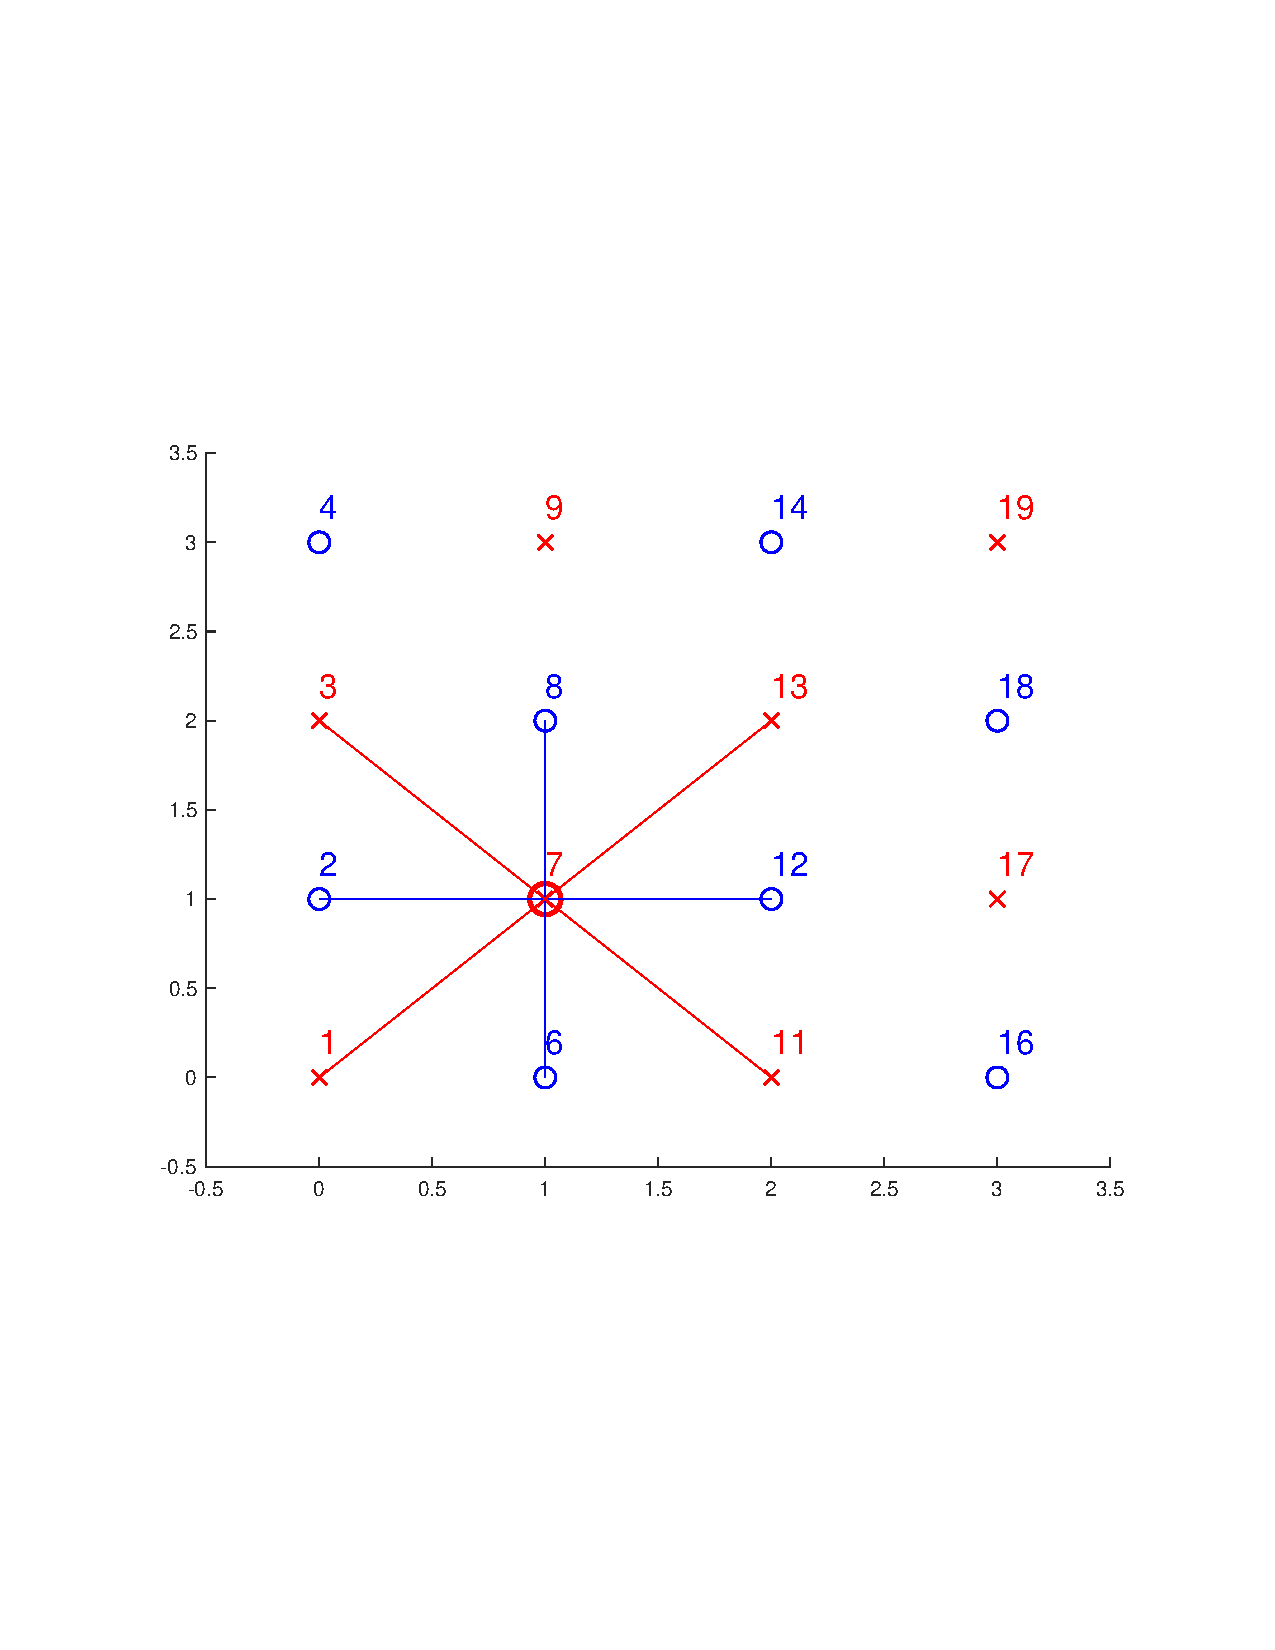
\includegraphics[width=7cm]{RRG_Ising_2D}
\caption{\bf Illustration of the RG scheme for 2D Ising. 
}
\label{fig:rng:ising:2d} 
\end{center}
\end{figure}
%
The goal is again to decimate the lattice by integrating out sublattice B, i.e.
to compute the reduced density matrix for sub-lattice A.
The reduced density matrix on sub-lattice A is
%
\begin{align*}
\rho_{A} &= \sum_{\{S_{i}\}\in B} e^{-\beta H}
\end{align*}
%
To get an idea of one renormalization step,
we consider all terms of the hamiltonian that contain the spin on site 7, which is part of sub-lattice B.
%
\newcommand{\Snn}{{\cal S}^\text{nn}_{7}}
\newcommand{\Snnn}{{\cal S}^\text{nnn}_{7}}
\begin{align*}
-\beta H_{7} &= C + h S_{7} + K \Snn S_{7 }\\
\Snn &= S_{2} + S_{6} + S_{8} + S_{12}\;.
\end{align*}
%
Next we separate the contribution of this spin from the rest
%
\begin{align*}
\rho_{A} &= \sum_{\{S_{i}\}\in B / S_{7}} e^{-\beta H'} \cdot Z_{7}\\
Z_{7} &= \sum_{S_{7}} e^{-\beta H_{7}}
\end{align*}
% 
with $H'=H-H_{7}$ being the hamiltonian without site 7.
The trace over $S_{7}$ yields
%
\begin{align}\label{eq:Z:7a}
Z_{7}:=
\sum_{S_{0}} e^{C + S_{7}\big( K \;\Snn +h\big) }
&= e^{C} \cdot 2\cosh\big(K \Snn  +h  \big)\;.
\end{align}
%
We want to express this function again as
%
\begin{align*}
e^{- \beta \tilde H}\;.
\end{align*}
%
The most general exponential form for this expression, since $S_{i}^{2}=1$, is given by
%
\begin{align}\label{eq:Z7}
Z_{7}&= \exp\bigg(C' + h' {\cal S}_{7}	^{nn}\;.
+ \overline{K} \sum'_{ij}  S_{i}S_{j}  +
b \sum'_{ijk} S_{i}S_{j} S_{k}  + c \; S_{2}S_{6}S_{8}S_{12}\bigg)\;.
\end{align}
%
The indices in the sums are from the set $I^{nn}_{7} =\{2,6,8,12\}$,
and the prims indicate that  no indices must occur twice and all the indices shall be ordered, e.g. $S_{i}<S_{j}<S_{k}$. 
We have used the symmetry that \eq{eq:Z:7a}
is invariant against interchange of any two indices $i\leftrightarrow j$.
Otherwise , each product of spins would have its own prefactor.

In the double sum there are also the products  $S_{6} S_{8}$ and $S_{2} S_{12}$,
which belong to next-nearest neighbour sites on the decimated lattice, which only consists of sub-lattice A (blue circles). I.e. starting from nn coupling
the decimation also introduces nnn coupling and also terms with three and four spins.
The latter will turn out negligible but the nnn coupling is relevant. 
To obtain the parameter mapping in an RG step, we include the nnn terms also in the original hamiltonian, i.e. 
\begin{align*}
-\beta H_{7} &= C + S_{7} \qty(h  + K  \Snn +L \Snnn)\\
\Snn &= S_{2} + S_{6} + S_{8} + S_{12}\\
\Snnn &= S_{1} + S_{3} + S_{11} + S_{13}\;.
\end{align*}
%
Again, we separate the contribution of this spin from the rest


%
\begin{align*}
\rho_{A} &= \sum_{\{S_{i}\}\in B / S_{7}} e^{-\beta H'}\cdot Z_{7}\\
Z_{7} &= \sum_{S_{7}} e^{-\beta H_{7}}
\end{align*}
% 
The trace over $S_{7}$ now yields
%
\begin{align}\label{eq:Z:7}
Z_{7}&= e^{C} \cdot 2\cosh\big(K \Snn  + L \Snnn + h  \big)\;.
\end{align}
%
Here we have a problem, since $\Snnn$ contains spins of sublattice B (e.g. $S_{13}$)
that still need to be integrated out and that are also contained in the   
residual hamiltonian  $H'$. In this combination the sum over $S_{13}$ is not as trivial as
that over $S_{7}$, which we had before. Moreover, the complexity increases, as $Z_{7}$
also contains other spins of sub-lattice $B$ ($S_{1}$ say) and after the trace over $S_{13}$ the expression containing $S_{1}$ is getting even more complicated, etc..
Hence, to keep things manageable, we replace  $\Snnn$ at this point by its mean value, which is zero.
Then we are left with
%
\begin{align}\label{eq:Z:7b}
Z_{7}&= e^{C} \cdot 2\cosh\big(K \Snn  + h  \big)\;.
\end{align}
%
\blue{As we will see soon, that does not mean that the original nnn coupling has no influence at all.}
We can use the general exponential from of \eq{eq:Z7} again
%
\begin{align*}
Z_{7} &= \exp\bigg(C' + h' {\cal S}+ \overline K \sum'_{ij}  S_{i}S_{j}  +
b \sum'_{ijk} S_{i}S_{j} S_{k}  + c \; S_{2}S_{6}S_{8}S_{12}\bigg)\;.
\end{align*}
%
As before, the indices in the sums are from the set $I^{nn}_{7} =\{2,6,8,12\}$.
The term with 3 spins can equivalently be written as
%
\begin{align*}
\sum'_{ij} S_{i}S_{j}S_{k}   &= {\cal S} \cdot  S_{2}S_{6}S_{8}S_{12} 
\end{align*}
%
\emphasize{proof}{
%
\begin{align*}
\sum'_{ij} S_{i}S_{j}S_{k}  
&= S_{2}S_{6}S_{8}
+ S_{2}S_{6}S_{12}
 + S_{2}S_{8}S_{12}
  + S_{6}S_{8}S_{12}\\
  &= S_{2}S_{6}S_{8} S_{12}^{2}
+ S_{2}S_{6}S_{12} S_{8}^{2}
 + S_{2}S_{8}S_{12} S_{6}^{2}
  + S_{6}S_{8}S_{12} S_{2}^{2}\\
  &=S_{2} S_{6}S_{8}S_{12} \big( S_{12}+S_{8}+S_{6} +S_{2x^{}}\big)
\end{align*}
}

So we have the constraint
%
\begin{align}\label{eq:constr}
C + \ln\bigg(2\cosh\big[K{\cal S} +h  \big]  \bigg)&=
C' + h' {\cal S} + \overline K \sum'_{ij} S_{i}S_{j}  +
\bigg(b{\cal S} + c\bigg) S_{1}S_{2}S_{3}S_{4}
\end{align}
%
Now we consider this constraint for all possible spin configurations:
%
\begin{align*}
1)&&(++++)&:&C + \ln\bigg(2\cosh\big[4 K+h  \big]  \bigg) &=
C' + 4 h'  + 6 \overline K   + \big(4b+c\big)\cdot 1 \\
2)&&(+++-)&:&C + \ln\bigg(2\cosh\big[2 K+h  \big]  \bigg) &=
C' + 2 h'  + 0 \overline K   + \big(2b+c\big)\cdot (-1) \\
3)&&(++--)&:&C + \ln\bigg(2\cosh\big[0K+h  \big]  \bigg) &=
C' + 0 h'  - 2 \overline K   + \big(0b+c\big)\cdot 1 \;
\end{align*}
%
Since the geometric position of the spins does not enter in \eq{eq:constr} we get the same equations if we permute the spins.

%
The remaining spin configurations
are obtained by the transformation $S_{i}\to - S_{i}$, which changes the sign in the terms with an odd number of spins. I.e. 3) is invariant, and for the other two we obtain
\begin{align*}
1')&&(----)&:&C + \ln\bigg(2\cosh\big[-4 K+h  \big]  \bigg) &=
C' - 4 h'  + 6 \overline K   + \big(-4b+c\big)\cdot 1 \\
2')&&(---+)&:&C + \ln\bigg(2\cosh\big[-2 K+h  \big]  \bigg) &=
C' - 2 h'  + 0 \overline K   + \big(-2b+c\big)\cdot (-1) \\
\end{align*}
%
We simplify these equations a bit further
\begin{align*}
1)&&(++++)&:& \ln\bigg(2\cosh\big[4 K+h  \big]  \bigg) &=
\Delta C + 4 h'  + 6 \overline K   + 4b+c \\
1')&&(----)&:& \ln\bigg(2\cosh\big[-4 K+h  \big]  \bigg) &=
\Delta C  - 4 h'  + 6 \overline K   -4b+c \\
2)&&(+++-)&:&\ln\bigg(2\cosh\big[2 K+h  \big]  \bigg) &=
\Delta C + 2 h'   - 2b-c \\
2')&&(---+)&:&\ln\bigg(2\cosh\big[-2 K+h  \big]  \bigg) &=
\Delta C - 2 h'     + 2b-c\\
3)&&(++--)&:& \ln\bigg(2\cosh\big[h  \big]  \bigg) &=
\Delta C - 2 \overline K   + c \;,
\end{align*}
%
with $\Delta C = C'-C$. 

%
When we add or subtract equation 1 and 1' and likewise for 2 and 2', we obtain
%
\begin{align*}
a)&:& \ln\bigg(4\cosh\big[4 K+h  \big] \cosh\big[4 K-h  \big] \bigg) &= 2\bigg( 
  \Delta C + 6\overline K +c   \bigg)\\
a')&:&  \ln\bigg(\cosh\big[4 K+h  \big]/ \cosh\big[4 K-h  \big] \bigg) &= 8\big( h' +b
 \big)\\
b)&:&2\ln\bigg(4\cosh\big[2 K+h  \big]\cosh\big[2 K-h  \big]  \bigg) &=
4\bigg( \Delta C -c \bigg)\\
b')&:&2\ln\bigg(\cosh\big[2 K+h  \big]/\cosh\big[2 K-h  \big]  \bigg) &=
8\bigg(h' -b \bigg)\;.
\end{align*}
Equation 3) yields
%
\begin{align*}
c)\Delta C +c   &=
\ln\bigg(2\cosh\big[h  \big]  \bigg) + 2 \overline K
\end{align*}
%
  
%
Inserting c) into a) gives
\begin{align*}
\tilde a)&:& \ln\bigg(4\cosh\big[4 K+h  \big] \cosh\big[4 K-h  \big] \bigg) &= 2
 \ln\bigg(2\cosh\big[h  \big]  \bigg)+ 16\overline K   \\
&&16 \overline K &= \ln\bigg(
\frac{\cosh\big[4 K+h  \big] \cosh\big[4 K-h  \big] }{\cos^{2}([h]}
  \bigg)
\end{align*}
%
We see that $\overline K$ only depends on $K$ and $h$.
If we add a') and b') we obtain
%
\begin{align*}
16 h' &=
\ln\bigg( 
\frac{\cosh\big[4 K+h  \big]\cosh^{2}\big[2 K+h  \big]}{\cosh\big[4 K-h  \big]\cosh^{2}\big[2 K-h  \big]  }
 \bigg)\;.
\end{align*}
%
Also $h'$ only depends on $h$ and $K$. Especially for $h=0$, we find $h'=0$. So 
the renormalization does not introduce a B-field, when we start with $B=0$. 

%%
%\begin{align*}
%e^{-16 \overline K} &= 
%\frac{\cosh^{2}(h)}{\cosh\big[4 K+h  \big] \cosh\big[4 K-h  \big] }
%=
%\frac{(e^{h}+e^{-h})^{2}}{(e^{4 K+h }+e^{-4 K-h}) (e^{4 K-h }+e^{-4 K+h}) }\\
%&=
%\frac{e^{2h} (1+e^{-2h})^{2}}{e^{8K}e^{2h}(1+e^{-8 K-2h}) (e^{-2h }+e^{-8 K}) }\\
%&=e^{-8K}
%\frac{(1+e^{-2h})^{2}}{(1+e^{-8 K-2h}) (e^{-2h }+e^{-8 K}) }\\
%e^{-16 h'} &=
%\frac{\cosh\big[4 K-h  \big]\cosh^{2}\big[2 K-h  \big]  }{\cosh\big[4 K+h  \big]\cosh^{2}\big[2 K+h  \big]}\\
%&=
%\frac{(e	^{4 K-h}+e	^{-4 K+h})  (e^{2 K-h}+e^{-2 K+h})^{2}   }
%{(e	^{4 K+h}+e	^{-4 K-h}) (e^{2 K-h}+e^{-2 K+h})^{2}   }\\
%&=
%\frac{e^{8K}(e	^{-h}+e	^{-8K+h})  (e^{-h}+e^{-4 K+h})^{2}   }
%{e^{8K}(e	^{h}+e	^{-8 K-h}) (e^{-h}+e^{-4 K+h})^{2}   }\\
%&=
%\frac{e^{3h}(e	^{-2h}+e	^{-8K})  (e^{-2h}+e^{-4 K})^{2}   }
%{e^{3h}(1+e	^{-8 K-2h}) (e^{-2h}+e^{-4 K})^{2}   }\\
%&=
%\frac{(e	^{-2h}+e	^{-8K})  (e^{-2h}+e^{-4 K})^{2}   }
%{(1+e	^{-8 K-2h}) (e^{-2h}+e^{-4 K})^{2}   };.
%\end{align*}
%
%%
%\begin{align*}
%e^{-16 \overline K} 
%&=e^{-8K}
%\frac{(1+e^{-2h})^{2}}{(1+e^{-8 K-2h}) (e^{-2h }+e^{-8 K}) }\\
%e^{-16 h'}
%&=
%\frac{(e	^{-2h}+e	^{-8K})  (e^{-2h}+e^{-4 K})^{2}   }
%{(1+e	^{-8 K-2h}) (e^{-2h}+e^{-4 K})^{2}   };.
%\end{align*}
In the following we will consider only the case $h=0$. Then we obtain  

%
\begin{align}\label{eq:ol:K}
\overline K &= \frac{1}{16}\ln(\cosh^{2}[4 K])
= \frac{1}{8}\ln(\cosh[4 K])\;.
\end{align}
%
Later on we will also need the derivative
%
\begin{align}\label{eq:der:ul:K}
\alpha(K) &= \dv{\overline K(K)}{K} =\frac{1}{2} \tanh(4 K)
\end{align}
%
For the determination for the other parameters for $h=0$ we have to solve

%
\begin{align*}
b)&\Rightarrow \overline{b}& \ln\bigg(2\cosh\big[2 K\big] \bigg) &=
\Delta a -c \tag{$\overline b$}\\
b')&\Rightarrow&0&= 8\big(h' -b \big)\tag{$\overline b'$}\\
c)&\Rightarrow\overline{c}& \ln(2) + 2 \overline K &=\Delta a +c   \tag{$\overline c$}
\end{align*}
%


We know already that $h=0$ also means $h'=0$ and according to $\overline b'$ this implies    $b=0$. 
I.e. the three-spin coupling  vanishes, which is reasonable, because without an external B-field no spin-direction  is favoured, i.e. the hamiltonian is invariant under the reversion of all spins. This symmetry would be violated by the three-spin coupling.
Finally, $\overline c$ - $\overline b$ yields
%
\begin{align}\label{eq:four:spin:term}
c &= \overline K  - \frac{1}{2}\ln(\cosh(2 K))
\end{align}
%



In addition, from $\overline c + \overline b$ we obtain
%
\begin{align*}
\Delta a &= \frac{1}{2}\qty( 2\ln(2) +  \ln(\cosh(2K)) +    2 \overline K )\;.
\end{align*}
%
Along with \eq{eq:ol:K} we obtain
%
\begin{align}\label{eq:Delta:a}
\Delta a &=   \ln(2) + \frac{1}{2}\ln(\cosh(2K))  + \frac{1}{8}\ln(\cosh(4 K)) \\
\Delta a &=   \ln(2 \cosh^{\frac{1}{2}}(2K)\cosh^{\frac{1}{8}}[4 K]) \;.
\end{align}
%


\subsubsection{First approximation, ignoring nnn interaction}
 
 
In \eq {eq:constr} we have the new two-spins interaction term in the decimated lattice, which is given by
%
\begin{align}\label{eq:E7}
E_{7}(S) :=
 \overline K \sum'_{ij} S_{i}S_{j} &=
 \overline K
\underbrace{
\qty(S_{2}S_{6}+S_{6}S_{12}+S_{12}S_{8}+S_{8}S_{2})
}_{\color{blue} = \text{nn terms in dec. lattice}}
+ \ldots\\
&+
\overline K
\underbrace{\qty(S_{2}S_{12}+S_{6}S_{8})}_{\color{blue} = \text{nnn terms in dec. lattice}}
\end{align}
%
This is the interaction that comes from the sum over $S_{7}$. 
Among others, there  is  a coupling between $S_{8}$ and $S_{12}$.
Integrating out $S_{13}$ also mediates a coupling between these spins. 
These contributions add up. Therefore, we 
have for the new nn coupling between site $8$ and $12$
%
\begin{align*}
K' &= 2 \overline K\;.
\end{align*}
%
Moreover, in addition to the nn coupling we also have a nnn
coupling in the decimated lattice. Both couplings 
support the same  (ferromagnetic) orientation. 
As a first approximation, we want to omit these terms and use 
a modified nn coupling instead.

We consider the isolated cluster with sites $2,6,8,12$ with $S_{7}$ being integrated out. For a perfect ferromagnetic alignment (all spins in the cluster equal +1)
we have for the energy of that cluster if we include the nnn term
%
\begin{align*}
E_{7}(S) &= 6 \overline K \;.
\end{align*}
%
Omitting the nnn term and using $\tilde K$ for the nn coupling instead, we find

%
\begin{align*}
\tilde E_{7}(S) &= 4 \tilde K \;.
\end{align*}
%
These energies shall be the same and we therefore use
%
\begin{align*}
\tilde K &= \frac{3}{2} \overline K\;. 
\end{align*}
%
As mentioned before, this coupling gets a factor two
by the integration of the neighbouring spins in the B sub-lattice.
Hence in this approximation we have
%
\begin{align}\label{eq:RG:2D:first}
K' &= 3 \overline K  = \frac{3}{8} \; \ln\bigg(  \cosh(4K)\bigg)\;.
\end{align}
%


%
\begin{figure}[htbp]
\begin{center}
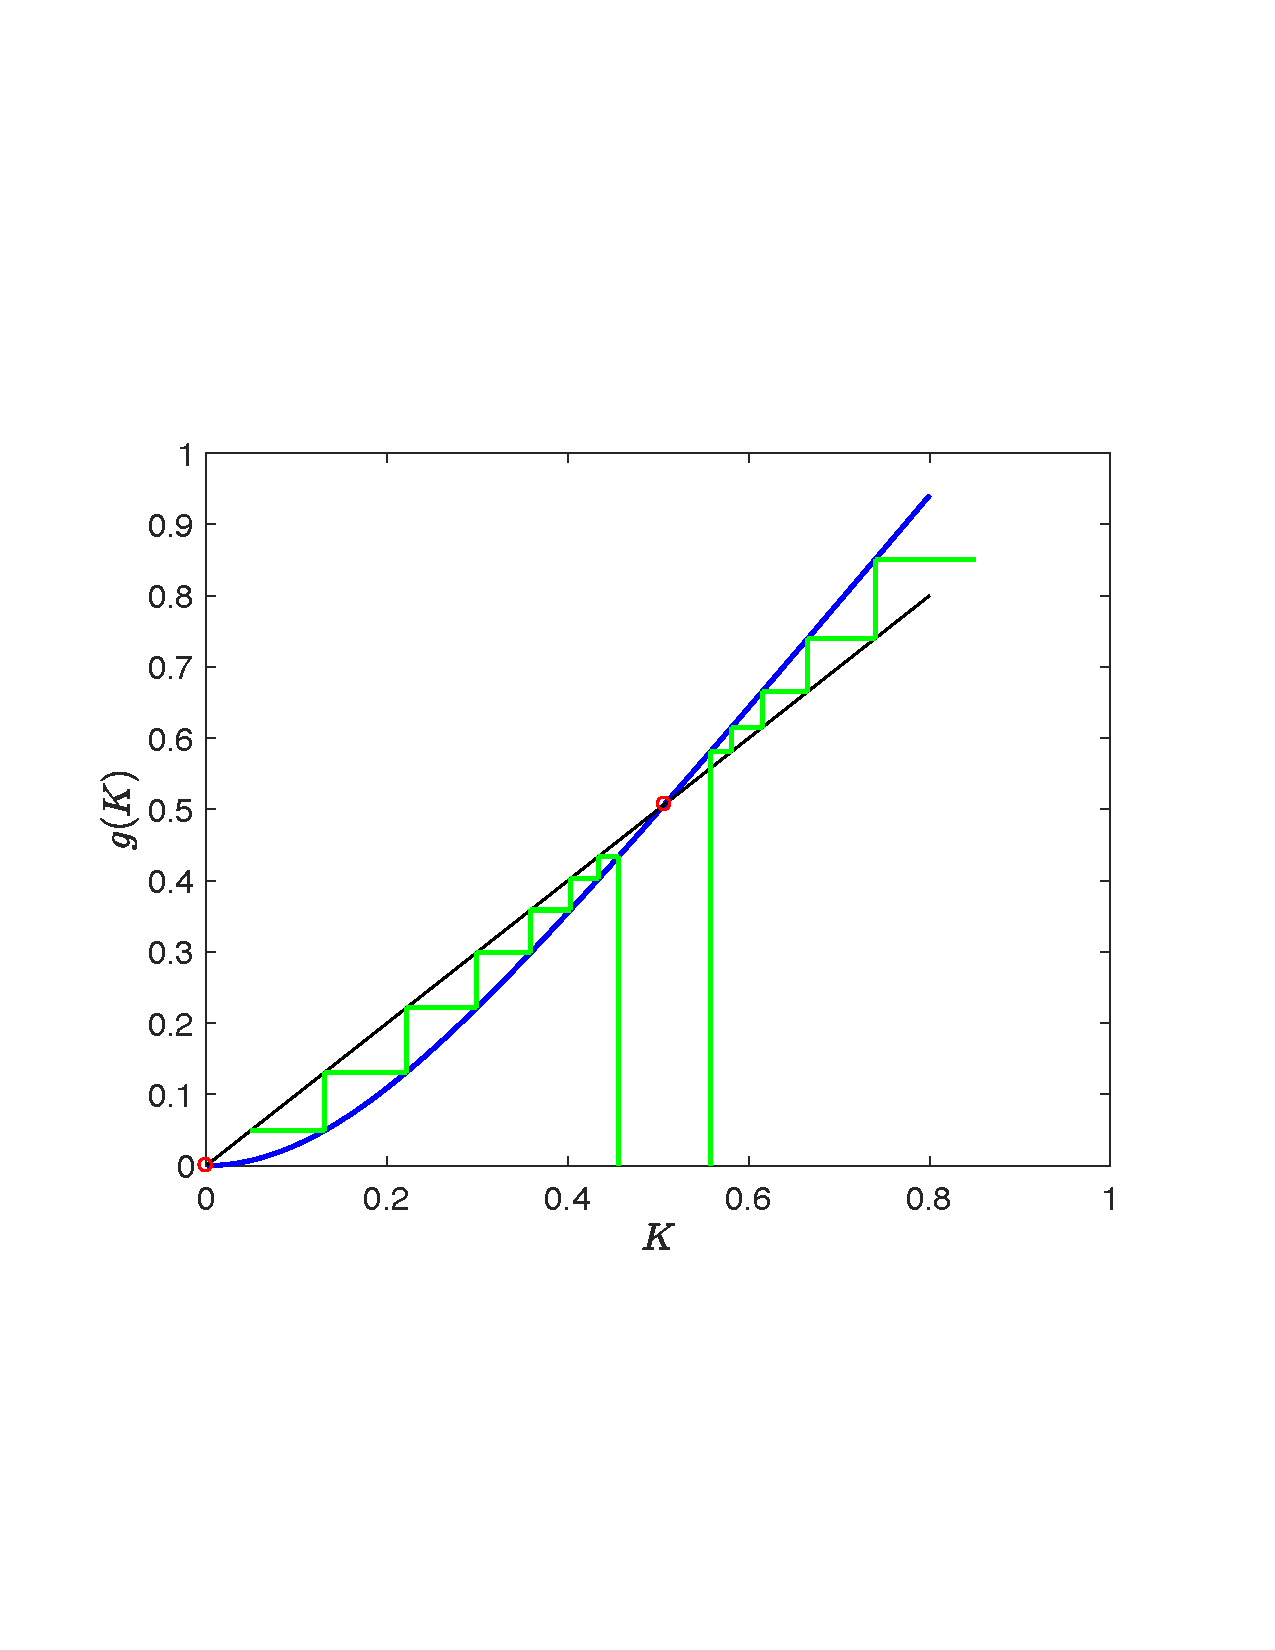
\includegraphics[width=7cm]{RNG_flow_2D}
\caption{\bf Flux of the renormalization iterations in the first approximation
described by equation (\ref{eq:RG:2D:first}).
}
\label{fig:rng:ising:2d}
\end{center}
\end{figure}



In \fig{fig:rng:ising:2d} the mapping of the coupling parameter $K$ during the renormalization
steps is depicted.
We find three fixed points, $K^*_{1}=0$, $K_{2}^{*}=\infty$, and $K^{*}_{3}=0.507$. 
The first two are the same as in the 1D case, \red{but with the important difference that now both fixed points are stable, while in the 1D case the
low-temperature fixed point $K^{*}=\infty$ was unstable.}
The $K^{*}=0$ fixed point is trivial and corresponds to $T=\infty$ where the correlations between neighboring spins vanish. The other fixed point ($K^{*}=\infty$) is a so-called critical fixed point as it describes the situation that the correlation length diverges for $T\to 0$
but there are nonetheless no fluctuations since all spins are perfectly aligned.
Only the third  fixed point describes a true \blue{critical point}. This one is   unstable. If we start with a physical parameter $K>K^{*}_{3}$ the interaction leads to $K=\infty$, while if we start with $K<K_{3}^{*}$ the iterations lead to $K=0$. Only starting precisely with $K=K^{*}_{3}$, the value of $K$ does not change.
So $K_{3}^{*} = \frac{J}{k_{B}T^{*}}$ corresponds to the phase transition. For $T<T^{*}$ 
($K>K^{*}_{3}$) the fixed point is $K\to \infty$, i.e. $T=0$ and hence long range order 
and in the other case the system behaves like $T=\infty$. 

The value $K^{*}_{3}=0.507$ has to be compared with the exact result
%
\begin{align*}
\beta^{*} J &= 0.4407\;.
\end{align*}
%
We have ignored so far the four-spin term. It has the coupling parameter $c$, which is given in 
\eq{eq:four:spin:term}. According to \eq{eq:RG:2D:first} we have
%
\begin{align*}
\overline K &= \frac{K'}{3}
\end{align*}

As the recursion equation for $K$ is independent of the other parameters, 
we can replace $K$ by its  fixed point values $K^{*}$ and we obtain
\begin{align}\label{eq:four:spin:term}
c &=  \frac{K^{*}}{3}  - \frac{1}{2}\ln(\cosh(2 K^{*})) = -0.053.
\end{align}
%
%
The result confirms that the four-spin coupling is much smaller than the two-spin terms
and can, therefore, be either ignored or taken into account perturbationally.





\subsubsection{Second approximation, including nnn interaction}


%
\begin{figure}[htbp]
\begin{center}
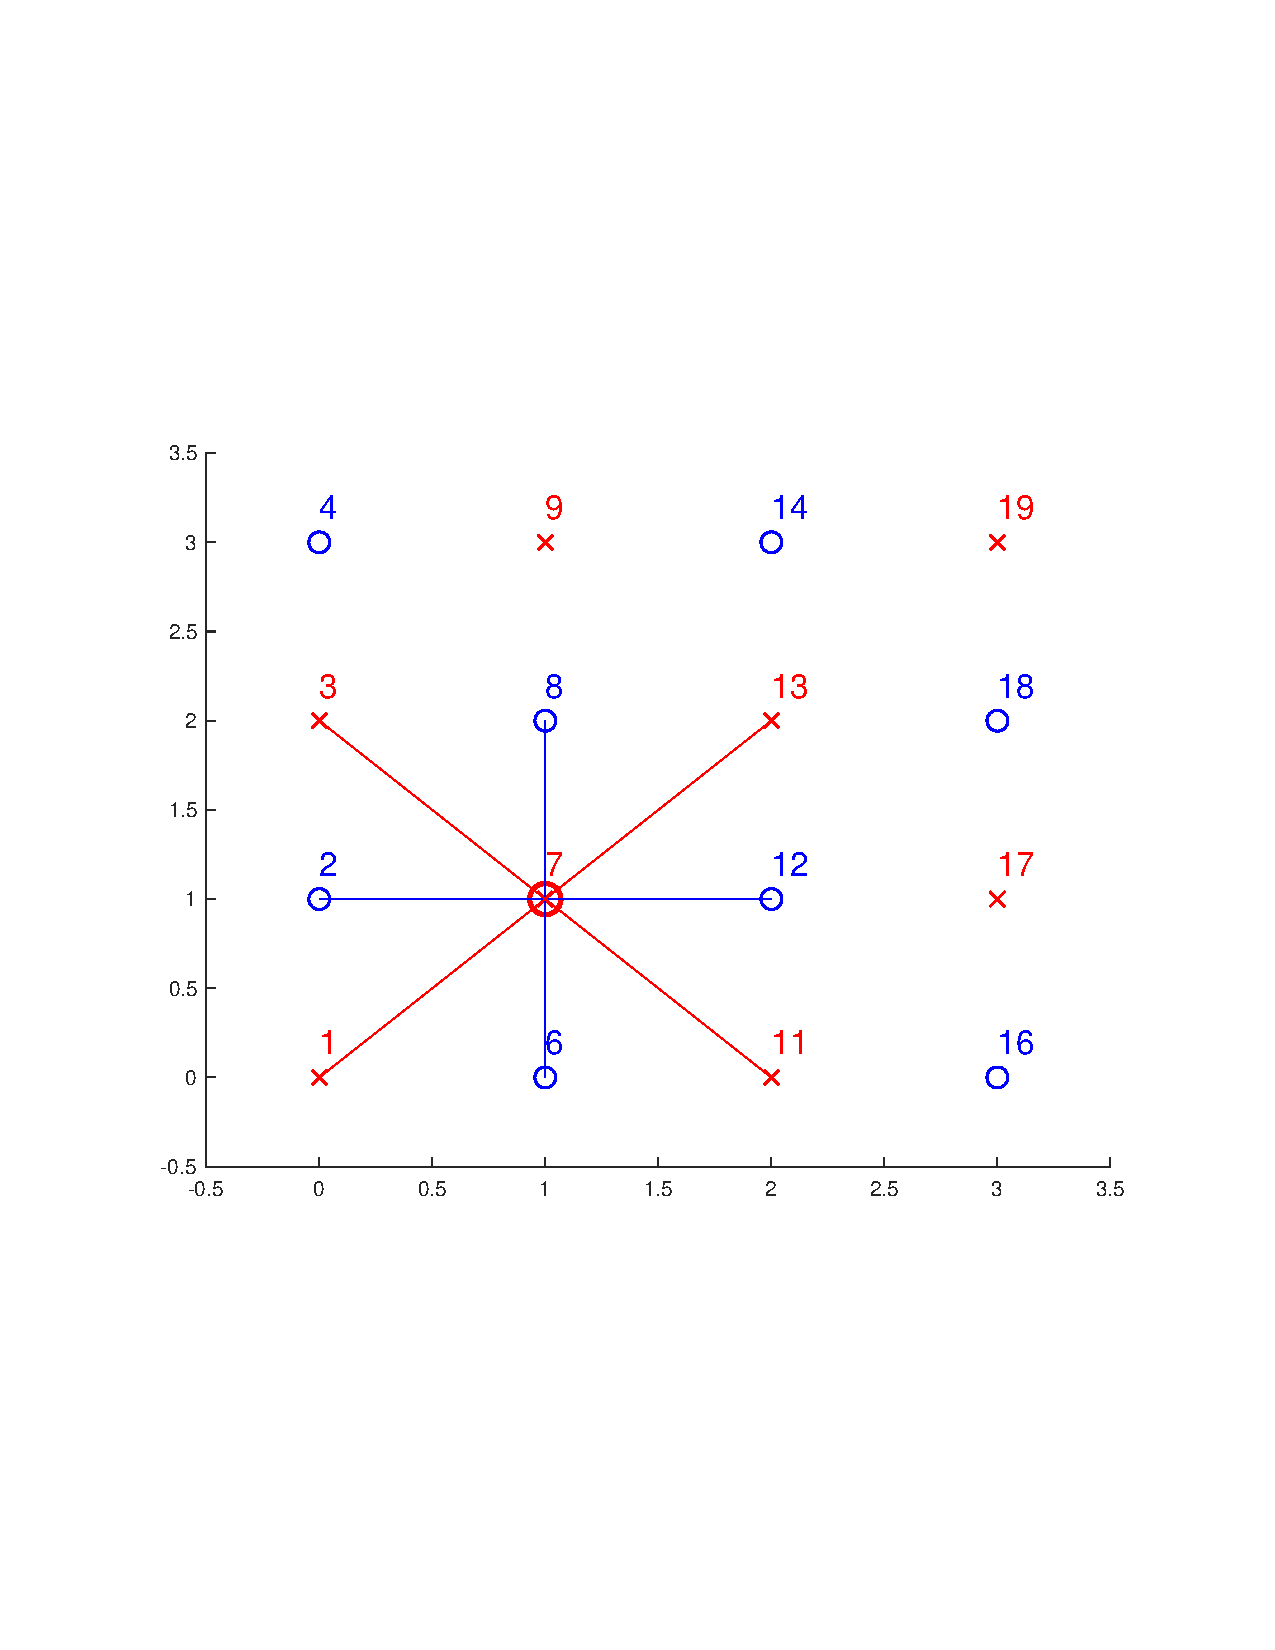
\includegraphics[width=7cm]{RRG_Ising_2D}
\caption{\bf Illustration of the RG scheme for 2D Ising. 
}
\label{fig:rng:ising:2d:b
} 
\end{center}
\end{figure}

As argued before the summation of $S_{7}$ and $S_{13}$ yield a nn 
coupling $2 \overline K$ for the nn spins $S_{8}$ and $S_{12}$, in the decimated lattice. In addition for the same spins, we still have the  nnn coupling $L$ of the original 
lattice, which is not modified by the summation over spins of the B sub-lattice.
Hence 
%
\begin{align}
K' &= 2 \overline K + L\;.
\end{align}
%
The  new nnn coupling in the decimated lattice (between $S_{2}$ and $S_{12}$, say),
is given by $\overline K$ 
\blue{(see second term on rhs of \eq{eq:E7}). The coupling of these spins  is only generated by summing over $S_{7}$; hence no factor 2)}. The total RG iteration for the parameters $K$ and $L$ is
%
\begin{align}\label{eq:RG:Ising:2D:b}
K' &= \frac{2}{8}\ln(\cosh[4K])    + L\\
L' &= \frac{1}{8}\ln(\cosh[4K])\;.
\end{align}
%
These equations have the following fixed points
\begin{align}\label{eq:RG:Ising:2D}
K^{*} &= \frac{2}{8}\ln(\cosh[4K^{*}])    + L^{*}\\
L^{*} &= \frac{1}{8}\ln(\cosh[4K^{*}])\;.
\end{align}
%
Inserting the second equation into the first gives
%
\begin{align*}
K^{*} &= \frac{3}{8}\ln(\cosh[4K^{*}])\;.
\end{align*}
%
This is the same fixed point equation as before in \eq{eq:RG:2D:first} , resulting in
$K_{1}^{*}=0, K_{2}^{*}=\infty$, and $K_{3}^{*}=0.507$.
For the unstable fixed point we have
%
\begin{align}
K^{*}_{3} &= 0.507\\
L^{*}_{3} &= \frac{K^{*}}{3} = 0.169\;.
\end{align}
%
Next we will analyse this fixed point in more detail and we will omit
the index for simplicity.
We consider the close neighbourhood of this fixed point and expand the iteration equation
%
\begin{align*}
K' &= 2 \overline K(K) + L\\
L' &= \overline K(K) \;,
\end{align*}
%
about the fixed point
%
\begin{align*}
K' &= 
\underbrace{2 \overline K(K^{*}) + L^{*}}_{\color{blue} = K^{*}} 
+ 2 \underbrace{
\eval{\frac{d \overline K(K)}{d K}}_{K^{*}}
}_{\color{blue} = \alpha^{*}}
\var  K
+ \var  L
\\
L' &= \underbrace{\overline K(K^{*})}_{\color{blue} = L^{*}} 
+ \underbrace{
\eval{\frac{d \overline K(K)}{d K}}_{K^{*}}
}_{\color{blue} = \alpha^{*}} \var  K
\end{align*}
%
The derivative is according to \eq{eq:der:ul:K}
%
\begin{align*}
\alpha^{*} &=  \frac{1}{2} \tanh(4 K^{*})
= 0.48297\;.
\end{align*}
%
Then with the definition  $\var \vv x = (\var K,\var L)^{T} = (K-K^{*},L-L^{*})^{T}$
we have
%
\begin{align*}
\var x'
&= 
\underbrace{
\mqty(2 \alpha^{*} & 1\\
\alpha^{*}&0
)
}_{\color{blue} = M}
\var x
\end{align*}
%
The matrix $M$ has the eigenvalues
%
\begin{align*}
\lambda_{\pm} &= \alpha^{*} \pm \sqrt{{\alpha^{*}}^{2} +\alpha^{*}}\\
\lambda_{+} &= 1.329282636504768\\
\lambda_{-} &= -0.363334404967798\;.
\end{align*}
%
and eigenvectors
%
\begin{align*}
\vv v_{\pm} &= 
\mqty(
\alpha^{*} \pm  \sqrt{{\alpha^{*}}^{2}+\alpha^{*}}\\\alpha^{*}
)\;.
\end{align*}
%

%
\begin{figure}[htbp]
\begin{center}
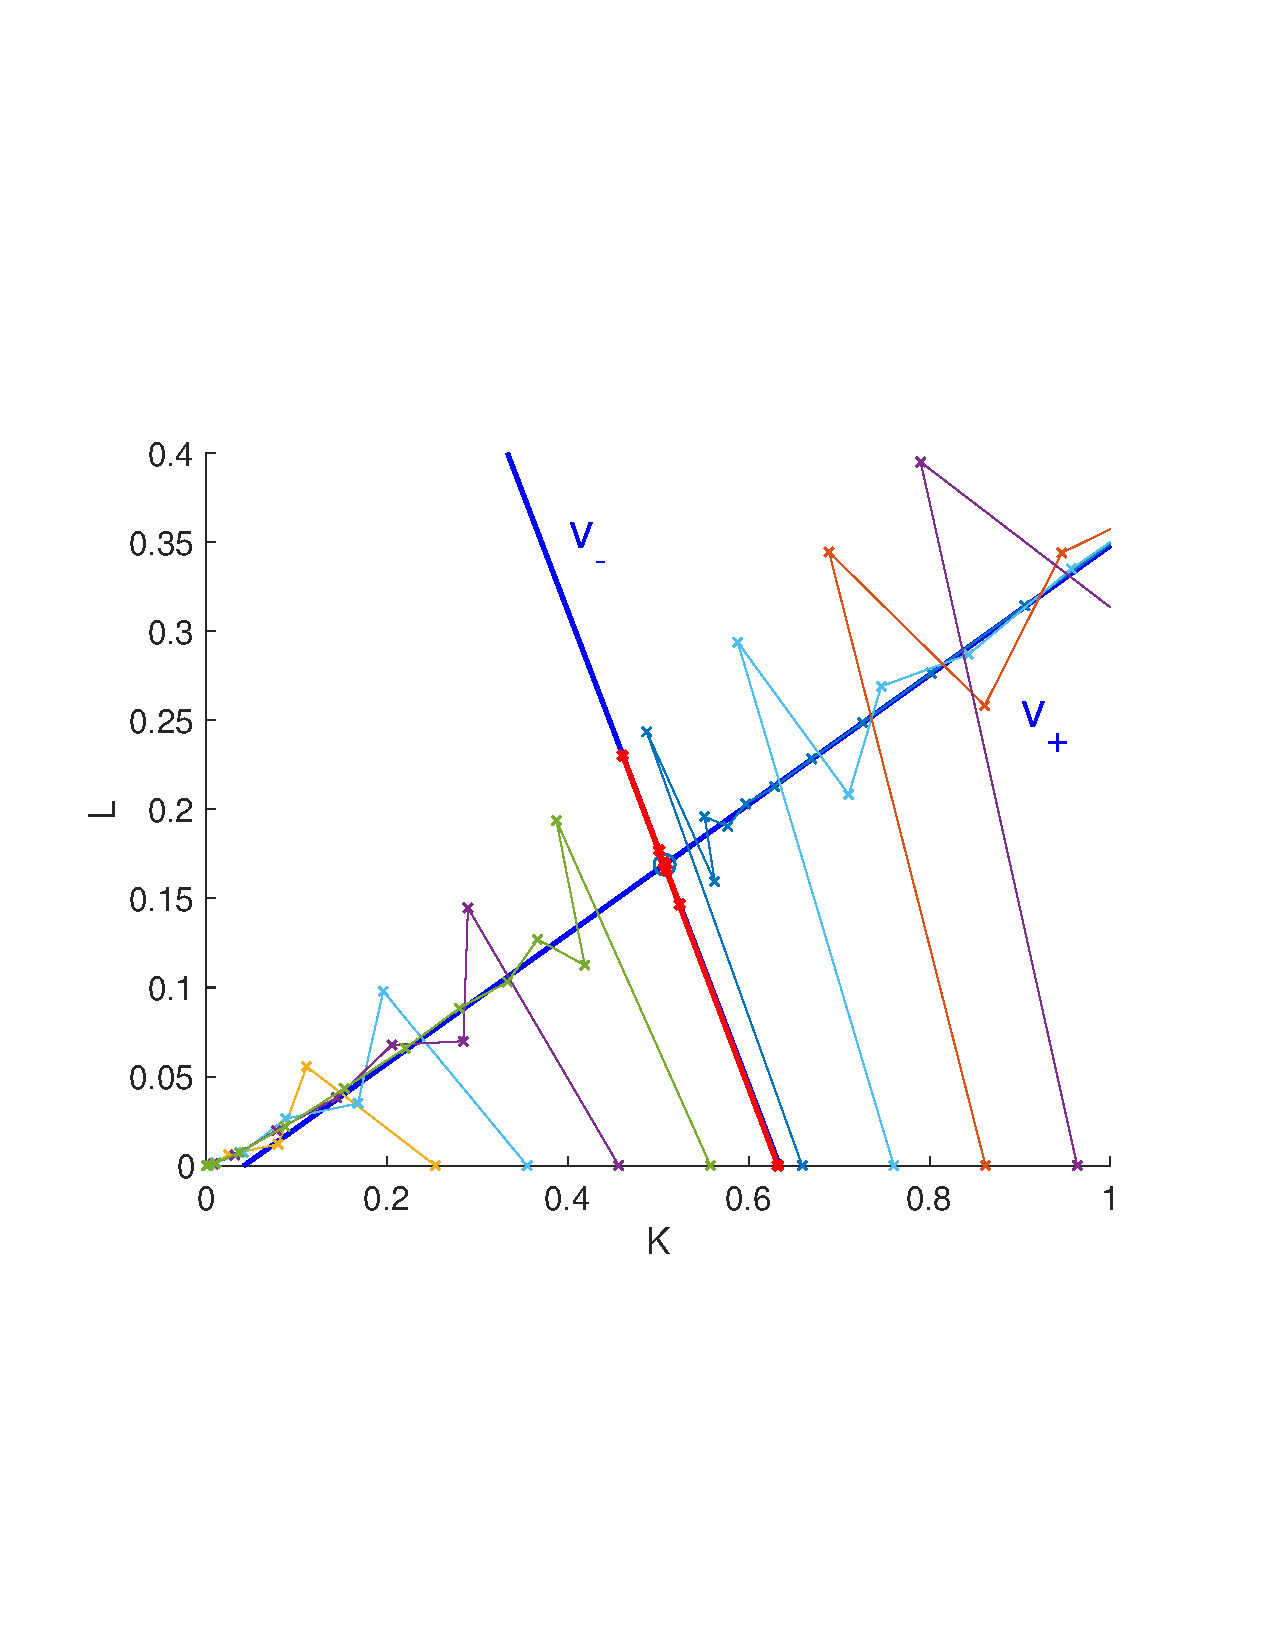
\includegraphics[width=7cm]{RRG_trajectory}
\caption{\bf Flux of the renormalization iterations in the second approximation
described by equation (\ref{eq:RG:Ising:2D:b}). 
All trajectories start at the physical values  $(K,0)$.
The blue solid lines represent the 
principle axes: $\vv x = \vv x^{*} + \lambda \vv v_{\pm}$. The red trajectory is obtained
when starting from $(K_{cr},0)$. Here $K_{cr}$ is chosen as follows: initially  $(K_{cr},0)
=(K^{*},L^{*}) + \eta \vv v_{-}$.   $\eta$ is chosen to fulfil the initial $L=0$ value.
}
\label{fig:rng:ising:2d:b}
\end{center}
\end{figure}

\subsubsection{Taylor expansion}

Often the RG-equation is approximated by assuming small parameters and employing only the 
leading order terms of the Taylor expansion about parameter values equal zero.

The Taylor expansion of $\frac{1}{8} \ln(\cosh(4x))$ gives
%
\begin{align*}
\frac{1}{8} \ln(\cosh(4x)) &= \frac{1}{8} \ln( 1 + \frac{(4x)^{2}}{2} +\ldots  )  = \frac{1}{8} \frac{(4x)^{2}}{2} + \ldots = x^{2}
\end{align*}
%
Then we obtain
%
\begin{align*}
\mqty(K^{*}\\L^{*})
&=
\mqty(
2 {K^{*}}^{2} & L^{*}\\
{K^{*}}^{2}&0
)
\end{align*}
%
with
%$
\begin{align*}
K^{*} &= 3 {K^{*}}^{2}\Rightarrow\qquad K^{*}=1/3\\
L^{*} &= 1/9
\end{align*}
%
In this case the critical value,  obtained numerically, reads $K_{cr} = 0.3921$. That is the K-value used for the initial point $(K,L=0)$ that separates the behaviour whether the trajectories converge towards $(0,0)$
or diverge. 

\begin{comment}

%
\begin{align*}
\mqty(\var K'\\\var L')
&=
\mqty(
4 K^{*} & 1\\
2 K^{*}&0
)
\mqty(\var K\\\var L)
=
\mqty(
\frac{4}{3} & 1\\
\frac{2}{3}&0
)
\mqty(\var K\\\var L)
\end{align*}
%

\end{comment}

%\begin{comment}

 
%



\section{Scaling and critical exponents}

To illustrate this idea we consider again the first approximation (ignoring the nnn
iterations). The iteration equation  was given in
\eq{eq:RG:2D:first} by
%
\begin{align*}
K' &= \frac{3}{8} \ln\qty( \cosh(4K)  ) := R(K)\;:
\end{align*}
%
We consider recursion steps in the vicinity of the fixed point.
We start out from the recursion relation for $K = K^{*}+\var K$
%
\begin{align*}
K' &= R(K) =R(K^{*}) + \underbrace{
\eval{\frac{d}{dK} R(K)}_{K=K^{*}}
}_{\color{blue} = \lambda}\;\var K\\
\Rightarrow\qquad \var K' &= \lambda \var K\;.
\end{align*}
%
The derivative yields
\begin{align}\label{eq:lambda}
\lambda &= \frac{3}{2} \tanh(4 K^{*}) = 1.4489\;.
\end{align}
%
In the present decimation scheme the length is scaled by $b=\sqrt{2}$. 
If we choose a different decimation factor $b$ also $\lambda$ will change, i.e.
%
\begin{align*}
\lambda &= \lambda(b)\;.
\end{align*}
%
When we perform 2 successive decimation steps  we have 
%
\begin{align*}
\var K'' &=\lambda(b) \var K' = \qty(\lambda(b))^{2} \var K\;.
\end{align*}
%
On the other hand, we could have performed the two decimation steps as one combined step of a new decimation scheme with $b'=b\cdot b$, then
%
\begin{align}
\var K'' &=\lambda(b') \var K\;,\nonumber \\
\Rightarrow\qquad \lambda(b^{2}) &= \lambda^{2}(b)\;\label{eq:RG:b}
\end{align}
%
The last equation requires
%
\begin{align*}
\lambda(b) &= b^{y}\;,
\end{align*}
%
where $y$ is a parameter that depends on the underlying physical system but not on $b$;
otherwise \eq{eq:RG:b} would not hold. For the present decimation scheme $b=\sqrt{2}$ and 
$\lambda=1.4489$ (see \eq{eq:lambda}), resulting in 
%
\begin{align*}
y &= \frac{\ln(\lambda)}{\ln(\sqrt{2})} = 1.070\;.
\end{align*}
%


\subsubsection{Correlation length}
We have

%
\begin{align*}
\var K &= K - K_{c} = \frac{J}{k_{B} } \qty(\frac{1}{T} - \frac{1}{T_{c}})
= \frac{J}{k_{B} T} \qty(\frac{T_{c}-T}{T_{c}}) = K \varepsilon \approx K_{c} \varepsilon\;.
\end{align*}
%
From the relation
%
\begin{align*}
\var K' &= b^{y} \var K
\end{align*}
%
we obtain
\begin{align}\label{eq:epsilon}
\varepsilon' &= b^{y} \varepsilon\;.
%\text{or rather } {\varepsilon'}^{-\nu} &= b^{- \nu y} \varepsilon^{-\nu}\;.
\end{align}
%
Moreover, close to $T_{C}$ we have generally
%
\begin{align*}
\frac{\xi}{a} &\sim \varepsilon^{-\nu}
\end{align*}
%
and in the decimated system similarly
%
\begin{align*}
\frac{\xi'}{a'} &\sim {\varepsilon'}^{-\nu}\;,
\end{align*}
%
where $a$ and $a'$ is the lattice constant in the corresponding system.
Then \eq{eq:epsilon} yields
%
\begin{align*}
\frac{\xi'}{a'} &\sim  {\varepsilon'}^{-\nu} =  b^{-\nu y}\;\varepsilon^{-\nu}\sim   b^{-\nu y}\;\frac{\xi}{a}\\
\Rightarrow\qquad \xi' &=  \underbrace{
\frac{a'}{a}
}_{\color{blue} = b (def.)} b^{- \nu y} \;\xi\\
\xi' &= b^{1 - \nu y} \;\xi\;.
\end{align*}
%
On the other hand, on approaching the fixed point the correlation length is converged and does not change. I.e.
%
\begin{align*}
\xi^{*} &= b^{1 - \nu y} \;\xi^{*}\;.
\end{align*}
%
Hence,
%
\begin{align*}
\nu y  &= 1\\
\nu &= \frac{1}{y} = 0.9346\;.
\end{align*}
%
Compared to the exact result ($\nu=1$) for the critical exponent the RG result is not so bad.




\subsubsection{Free energy and specific heat (a bit tricky, will be discussed later)}



Next we want to compute the critical exponent of the specific heat from the free energy 
%
\begin{align}\label{eq:CV:a}
C_{V} &= -T \eval{\pdv{F}{T}}_{V}\;.
\end{align}
%
For the critical exponent which is introduced in  \eq{eq:heat:capacity} as
%
\begin{align*}
C_{V}&\simeq  \abs{\varepsilon}^{-\alpha}
\end{align*}
%
we only need the close neighbourhood of the phase transition.
Hence the factor $T$ in \eq{eq:CV:a} can be replaced by $T_{C}$.
Moreover, we have
%
\begin{align*}
F &= - k_{B} T N \underbrace{
\frac{\ln(Z(K,N))}{N}
}_{\color{blue} := f(K,N)}\;.
\end{align*}
%
Also here the prefactor $T$ can be replace by $T_{C}$ as it does not modify the critical behaviour. So we have
%
\begin{align*}
C_{V} &\sim \pdv[2]{f}{T} \sim |\varepsilon|^{-\alpha}\;.
\end{align*}
%
We recall
%
\begin{align*}
\varepsilon &= \frac{T-T_{C}}{T_{C}}\;,
\end{align*}
%
which yields $f(\varepsilon,N)$ has to have the following behaviour near the phase transition
 %
\begin{align}
\pdv[2]f(\varepsilon,N) &\sim |\varepsilon|^{-\alpha}\nonumber\\
\Rightarrow\qquad f(\varepsilon,N) &\sim |\varepsilon|^{2 -\alpha}\;.
\label{eq:f:epsilon}
\end{align}
%
The integration would also yield a contribution $c + d \;\varepsilon$, which is, however, irrelevant for the critical behaviour.


Next we need to compute $f$.
We start out with the partition function  in the physical parameters 
%
\begin{align*}
Z(K,N) &= \sum_{\{S_{i}\}_{i=1}^{N}} e^{K \sum_{\avg{ij}} S_{i}S_{j}}\;.
\end{align*}
%
After one decimation we have 
%
\begin{align*}
Z(K,N) &= e^{\Delta a N } \sum_{\{S_{i}\}_{i=1}^{N/2}} e^{K' \sum_{\avg{ij}} S_{i}S_{j}}
= e^{\Delta a N } Z(K',N/2)\;.
\end{align*}
%
For the quantity $f(K) := \ln(Z(K,N))/N$ we obtain
%
\begin{align*}
f(K,N) &= \frac{\ln(Z(K,N))}{N} \\
&=\frac{\Delta a N + \ln(Z(K',N/2))}{N}\\
&=\Delta a +  \frac{1}{2} \underbrace{
\frac{\ln(Z(K',N/2))}{N/2}
}_{\color{blue} = f(K',N/2)}
\end{align*}




% 
Since $F=-k_{B} T \ln(Z)$  is an extensive quantity, $f(K,N)$ is independent 
of $N$. So we have
%
\begin{align*}
f(K) &= \Delta a + \frac{1}{2} f(K')\\
f(K') &= 2 f(K) -\Delta a
\end{align*}
%
Inserting \eq{eq:Delta:a} yields
\begin{align}\label{a}
f(K') &= 2 f(K) -   \ln(2 \cosh^{\frac{1}{2}}(2K)\cosh^{\frac{1}{8}}[4 K]) \;.
\end{align}
The second term is analytic and cannot lead to a critical behaviour. The only relevant, singular part $f_{s}$ behaves like
%
\begin{align*}
f_{s}(K') &= 2 f_{s}(K) = b^{d} f_{s}(K)\;.
\end{align*}
%
The scaling factor $b=\sqrt{2}$ and the spatial dimension is $d=2$. Or rather
%
\begin{align*}
f_{s}(K) &= b^{-d} f_{s}(K')\;.
\end{align*}
%
Close to the phase transition we have 
%
\begin{align*}
K &= K^{*} +\var K\\
K' &=  R(K^{*}) +\underbrace{
 \eval{\dv{R(K)}{K}}_{K=K^{*}}
}_{\color{blue} = \lambda}\;\var K\\
\var K' &= \lambda \;\var K
\end{align*}
%
As discussed before we have $\lambda=b^{-y}$ and hence
%
\begin{align*}
\var K' &= b^{y} \;\var K = b^{y} K^{*} \varepsilon
\end{align*}
%
So we have
%
\begin{align*}
f_{s}(K) &= b^{-d}\;f_{s}(K^{*} + b^{y} K^{*} \varepsilon)\\
 &= b^{-d}\;f_{s}(K^{*}[1 + b^{y}  \varepsilon])\;.
\end{align*}
%
This relation has to be valid for any decimation scheme, or rather $b$; so we can choose
%
\begin{align*}
b &= |\varepsilon|^{-1/y}
\end{align*}
%
resulting in 
%
\begin{align*}
f_{s}(K) &= b^{-d}\;f_{s}(K^{*} + b^{y} K^{*} \varepsilon)\\
 &= |\varepsilon|^{d/y}\;\underbrace{
f_{s}(K^{*}[1 +  \frac{\varepsilon}{|\varepsilon|}])
}_{\color{blue} = const}\;.
\end{align*}
%
So we have
%
\begin{align*}
f(\varepsilon,N)&\sim  |\varepsilon|^{d/y}\;.
\end{align*}
%
Comparison with \eq{eq:f:epsilon} yields
%
\begin{align*}
2 - \alpha &= \frac{d}{y}\\
\alpha &= 2 - \frac{d}{y}\;.
\end{align*}
%
Inserting the numerical value from \eq{} gives
%
\begin{align*}
\alpha &= 0.131\;.
\end{align*}
%
The exact value is $\alpha=0$ corresponding  to a logarithmic divergency.
While the mean field result of \eq{spec:heat:MFA} gave constant specific heat 
when approach from below $T_{C}$ and $C_{V}=0$ above $T_{C}$.


%\chapter{Percolation}
%commented out Feb 2024



